\section{Results Discussion}
To verify that our suppression of the spider through Gaussian division does not only work on the single data we have used until now, we perform the suppression on different images of HD142527. The data is taken in P2-mode, in this mode the ghosts and the possible exoplanets do not wander, but the spiders do. \\
Figure \ref{fig:Ghost2_apertures} (a) shows the calculated aperture flux from ghost 2 of the different images at different stages, starting with the original image, then transforming it to the $r$-$\varphi$ plane, flattening it and suppressing first the central radial frequencies and then all low frequencies. We observe that overall the aperture flux increases throughout the different steps and that it changes also during the warping due to the fact, that the ghost is not perfectly at the radial center, but it seems as if this step also slightly enhances the aperture flux. This is probably due to the fact that the ghost is in the lower part of the radial regime, so this is where, due to the warping, additional pixels need to be added which may result in an increase of the aperture flux. The flattening does not change the aperture flux much.\\
For a closer investigation on the suppression, we have a look at figure \ref{fig:Ghost2_apertures} (b), where we plotted the change of the aperture flux in percent and used the flattened image as reference. We observe that the suppression of the central radial frequency is the more important and the suppression of the other lower frequencies do not change much. We observe an overall increase of the aperture flux, but there are two images where the aperture flux decreased, namely at $x=3$ and $x=9$, and for the image $x=6$ the change is a lot smaller than for the rest. Here we need to keep in mind, that the position of the spiders move and that these results should depend on the distance between the ghost and the spiders. \\
We find that there are two different explanations for these cases where we have a decrease in aperture flux. One reason is that since the suppression tries to suppress the signal of the spiders, it should not change the aperture flux of the ghost, if it is not in a regime where it feels the influence of the spider. Indeed ghost 2 has the largest distance to the spiders in the image data $x=9$ and is therefore outside of the regime, where the spiders have an effect on its flux. However this result also could mean that this kind of spider suppression worsens the aperture flux a bit when we are looking at objects which are not close to any spiders.\\
An other reason for a decrease of the aperture flux (or almost no change) is that our method does not manage to suppress the spiders completely, especially in the center of the spider signal, there is no big change achieved by our suppression. This means that if the ghost and the spider overlap too much, we do not gain something from the suppression. In the image data of $x=3$ and $x=6$ the ghost is almost lying exactly on top of the spider.\\
So far we can say that the suppression by division is mainly useful if we want to find objects which are close by the spider, but not too close. \\
\begin{figure}[H]
	\centering
		\subfigure[]{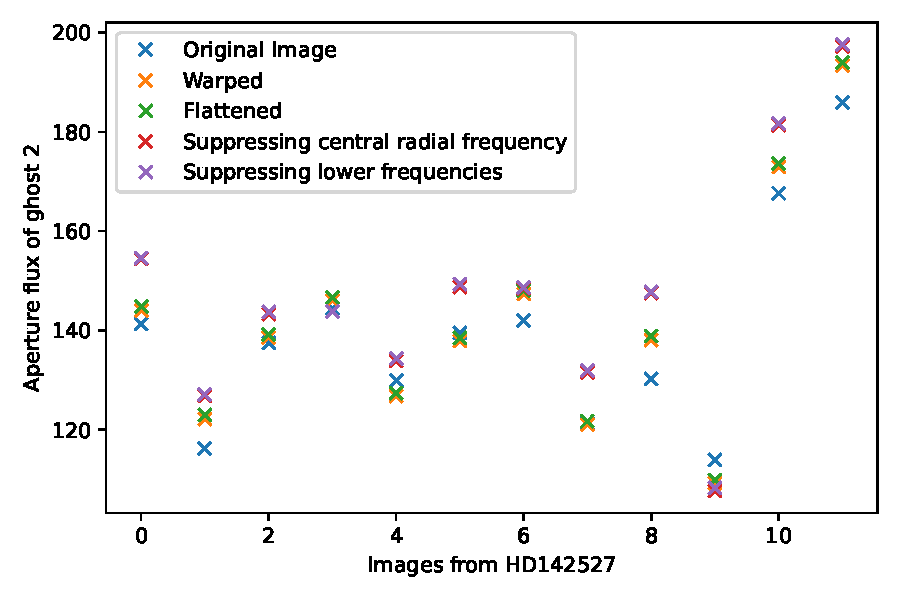
\includegraphics[width=0.49\textwidth]{pics/Ghost2_apertures.pdf}}
		\subfigure[]{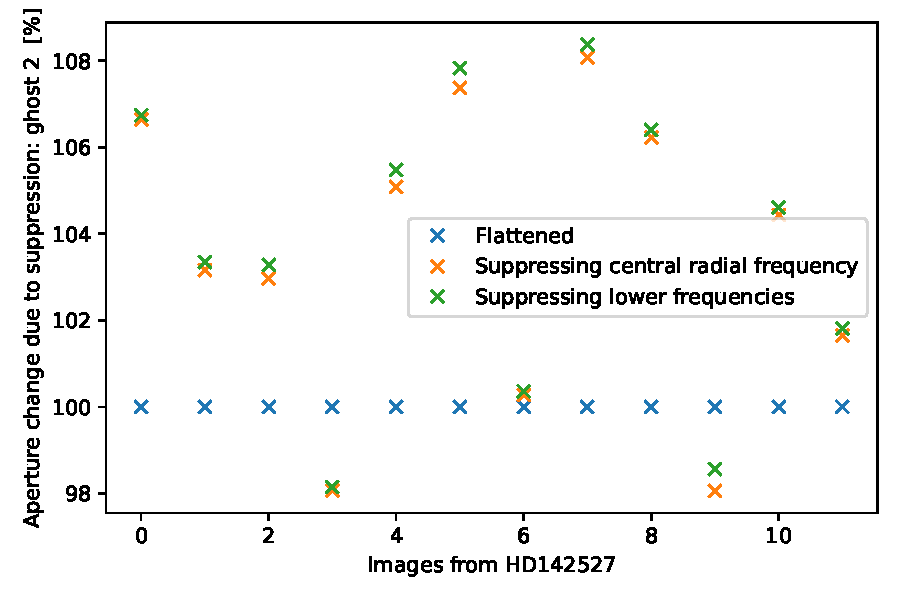
\includegraphics[width=0.49\textwidth]{pics/Ghost2_apertures_perc.pdf}}
\caption{The aperture flux of ghost 2 is calculated after each step from the transformation to the final suppression by Gaussian division (a). The aperture change due to the suppression in percent is shown in (b), where we use the flattened image as reference.}
\label{fig:Ghost2_apertures}
\end{figure}
For ghost 1 we have made the same plots as for ghost 2 which are shown in figure \ref{fig:Ghost1_apertures}. In contrast to before, where the overall aperture flux increased, we now observe a decrease in aperture flux. Mainly this decrease is caused by the warping, but this was to be expected. Since ghost 1 is in this case in the outer radial regime, pixels need to be taken together for the warping which results in a decrease of the aperture flux. Additionally the ghost gets a little bit elongated in radial direction which could also lead to a decrease in aperture flux during the suppression, since the ghost gets a form which is a little bit similar to a spider. The flattening however does not change the aperture flux much.\\
For a closer investigation on the suppression, we have a look at figure \ref{fig:Ghost1_apertures} (b). We observe that the suppression of the lower frequencies always lead to a decrease in aperture flux. The suppression of the central radial frequency mostly also leads to a decrease, only for $x=0$, $x=10$ and $x=11$ we observe an increase in aperture flux.\\
As we already observed before, the suppression only leads to an increase of the aperture flux, if the object is close enough at a spider so that it feels its influence. For the images where we observe an increase, this is also the case, whereas in all other images, the ghost is just too far away from the spiders.\\
\begin{figure}[H]
	\centering
		\subfigure[]{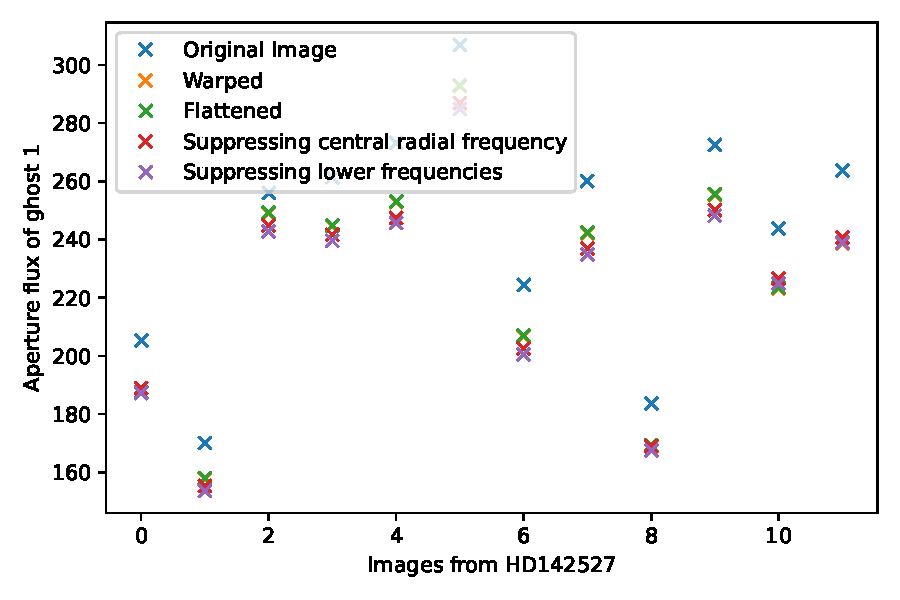
\includegraphics[width=0.49\textwidth]{pics/Ghost1_apertures.pdf}}
		\subfigure[]{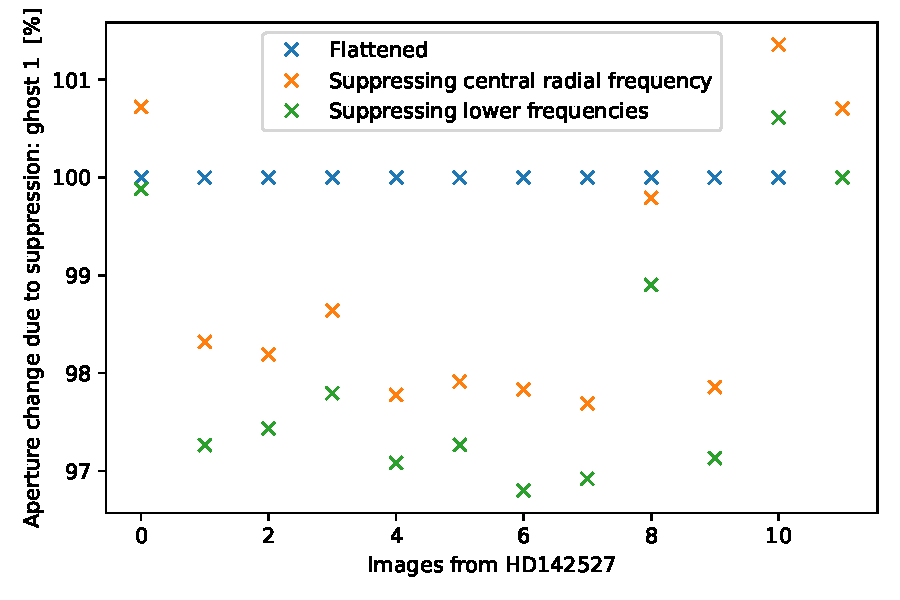
\includegraphics[width=0.49\textwidth]{pics/Ghost1_apertures_perc.pdf}}
\caption{The aperture flux of ghost 1 is calculated after each step from the transformation to the final suppression by Gaussian division (a). The aperture change due to the suppression in percent is shown in (b), where we use the flattened image as reference.}
\label{fig:Ghost1_apertures}
\end{figure}
Additionally to the calculation of the aperture flux of the ghosts we have also looked at a PSF (one which is approximately $10^{-6}$ times less bright then the star). The position of the PSF is marked in figure \ref{fig:HDimg_PSF}. The chosen position of the PSF is such that in our data-set it never comes close to one of spiders. 
\begin{figure}[H]
	\centering
		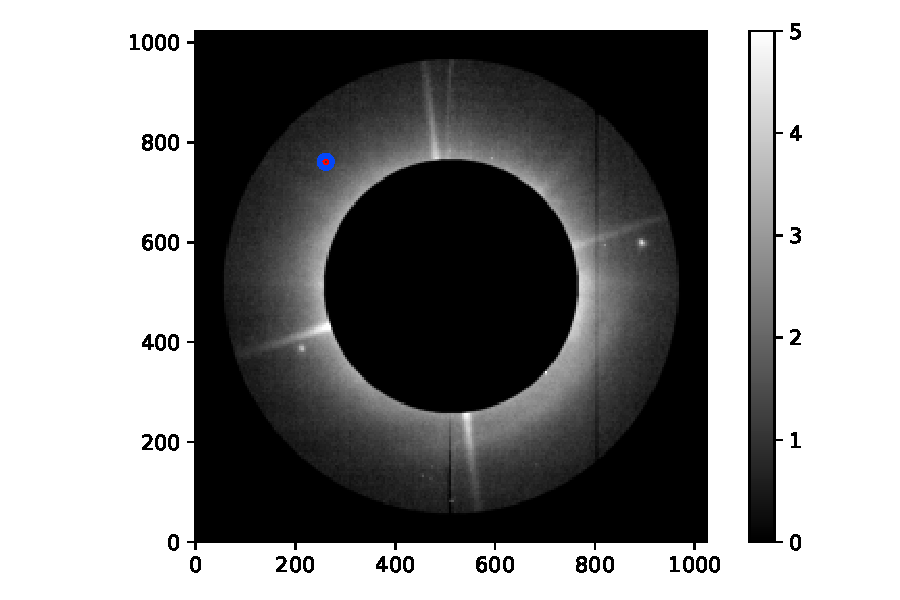
\includegraphics[width=0.7\textwidth]{pics/HDimg_PSF.pdf}
		\caption{We insert a PSF into the image of HD142527. The position of the PSF is marked in the image above, where we only look at the region between $R=254-454$.}
		\label{fig:HDimg_PSF}
\end{figure}
For this PSF we also look at the same plots as we did for ghost 1 and 2. The plots are shown in figure \ref{fig:PSF1000_apertures}. We see that due to the fact that the PSF has such a low intensity the aperture fluxes are all quite small and some of them are even negative, which means that the signal of the noise is sometimes even larger than the one from the PSF. We see that the changes in aperture flux due to the different processes is actually quite small, however most of the aperture fluxes decrease a bit, especially due to the warping. Although this time the PSF is placed exactly in the center of the radius range. As before the flattening does not change the aperture flux much.\\
For a closer investigation on the suppression, we have a look at figure \ref{fig:PSF1000_apertures} (b). Here we need to be careful when we look at the percentages, since the aperture flux values are all close to zero and some even change from positive to negative values during the warping or the suppression, we observe quite large changes, when we look at the change in percentage. The aperture flux however did not change significantly. We see that we observe both increasing and decreasing fluxes which are caused by the suppression. Therefore the suppression does not seem to help for objects outside of the spiders regime. Also smoothing of the images which we observed due to the suppression does not seem to help much. \\
We find that the images which have the overall lowest brightness seem to be the one where the aperture flux increases the most during the suppression. A possible improvement would be to adjust the angular division width on the overall intensity of the image. \\
\begin{figure}[H]
	\centering
		\subfigure[]{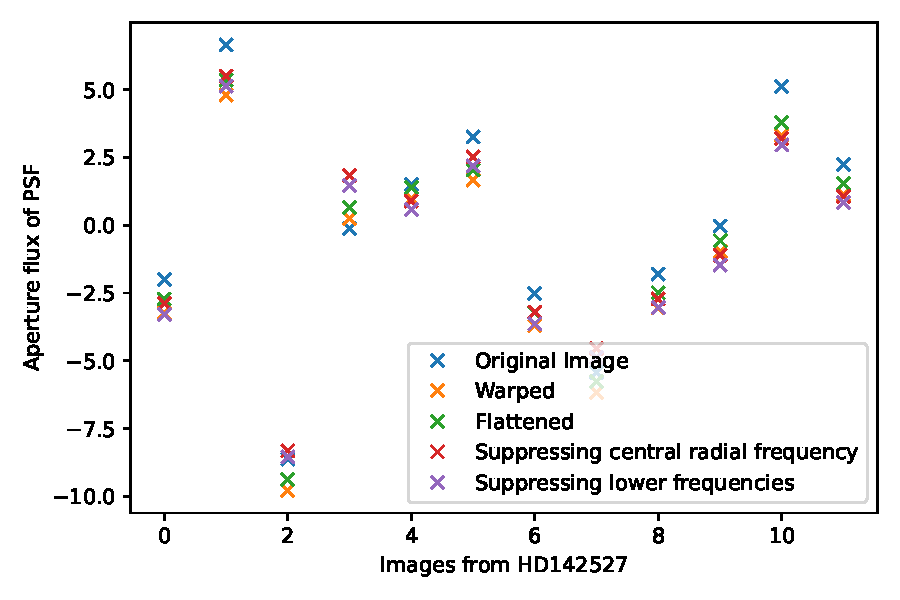
\includegraphics[width=0.49\textwidth]{pics/PSF1000_apertures.pdf}}
		\subfigure[]{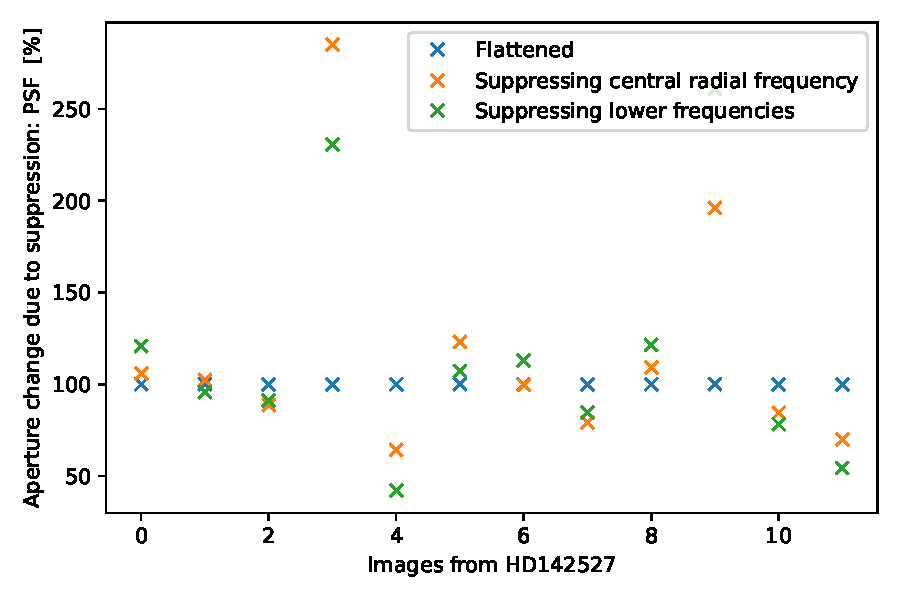
\includegraphics[width=0.49\textwidth]{pics/PSF1000_apertures_perc.pdf}}
\caption{The aperture flux of a PSF is calculated after each step from the transformation to the final suppression by Gaussian division (a). The aperture change due to the suppression in percent is shown in (b), where we use the flattened image as reference.}
\label{fig:PSF1000_apertures}
\end{figure}

